\documentclass[12pt,a4paper,titlepage]{article}
\usepackage{enumitem}
\usepackage{hyperref}
\usepackage{graphicx}
\usepackage{lab_style}
\usepackage{pdfpages}
\usepackage{eso-pic}

	\begin{document}
	
		\begin{center}
		
			\textsc{\large Faculty of Computers, Informatics and Microelectronics}\\[0.5cm]	
			\textsc{\large Technical University of Moldova}\\[1.2cm]
			\vspace{22mm}
			
			\textsc{\Large Digital Interactive Media and Software Development}\\[0.5cm]
			\textsc{\large Laboratory work \#1} \\[0.5cm]
			
			\newcommand{\KRule}{\rule{\linewidth}{0.5mm}}
			
			\vspace{10mm}
			\KRule \\[0.4cm]
			{\Large \bfseries Version Control Systems and Server Configuration }\\[0.4cm]
			\KRule \\[1.5cm]
			
			\vspace{30mm}
			\begin{minipage}{0.4\textwidth}
				\begin{flushleft}
					\emph{Authors:}\\
					Valentin \textsc{Suruceanu}
				\end{flushleft}
			\end{minipage}
			\begin{minipage}{0.4\textwidth}
				\begin{flushright}
					\emph{Supervisor:}\\
					Irina \textsc{Cojanu}
				\end{flushright}
			\end{minipage}\\[4cm]
			\vspace{5mm}
			\vfill							
		\end{center}
	
	\pagebreak
	\newpage
	 	\section*{Laboratory work \#1}
	 	
		\section{Purpose of the laboratory}
		Gain knowledge about basics of event-driven programming, understanding of window’s class and basic possibilities of Win32 API. Also she will try to understand and process OS messages.
		\section{Laboratory Work Requirements}
		\begin{itemize}
			\item \textbf{Basic Level (grade 5 - 6) you should be able to:}
		\begin{enumerate}
			\item Create a Windows application
      		\item In the middle of the window should be present the following text: "Done with Pride and Prejudice by student name". Replace student name with your name.
      		\item On windows resize, text should reflow and be in window's middle (vertically and horizontally)
      	\end{enumerate}
			\item \textbf{Normal Level (grade 7 - 8) you should be able to:}
      	\begin{enumerate}
    			\item Realize the tasks from \textit{Basic Level}.
    			\item Add 2 buttons to window: one with default styles, one with custom styles (size, background, text color, font family/size)
    			\item Add 2 text elements to window: one with default styles, one with custom styles (size, background, text color, font family/size)
          \end{enumerate}
			\item \textbf{Advanced Level (grade 9 - 10) you should be able to:}
		  \begin{enumerate}
    			\item Realize the tasks from \textit{Normal Level}.
    			\item Make elements to interact or change other elements (2 different interactions)  (ex. on button click, change text element color or position)
    			\item Change behavior of different window actions (at least 3). For ex.: on clicking close button, move window to a random location on display working space 
          \end{enumerate}
		\end{itemize}
		\clearpage
	\pagebreak
	\newpage
	\section{Laboratory Work Implementation}
	\subsection{Tasks and Points}
			\begin{enumerate}
				\item Clone the repository to the local machine
				\item Add .gitignore and README.md files
				\item Create folder MIDPS
				\item Create first folder (Lab\#1)
				\item Make a Commit when it's requaired
				\item Create a readme file
				\item Create the report
			\end{enumerate}
	\subsection{Laboratory work analysis}
	\newcommand\tab[1][1cm]{\hspace*{#1}}
			\tab \url{https://github.com/emptyshell/MIDPS.git}
	\subsection{Prove your work with screens}
	\begingroup
	\catcode`\#=12
	\begin{figure}[hb!]
	\centering
	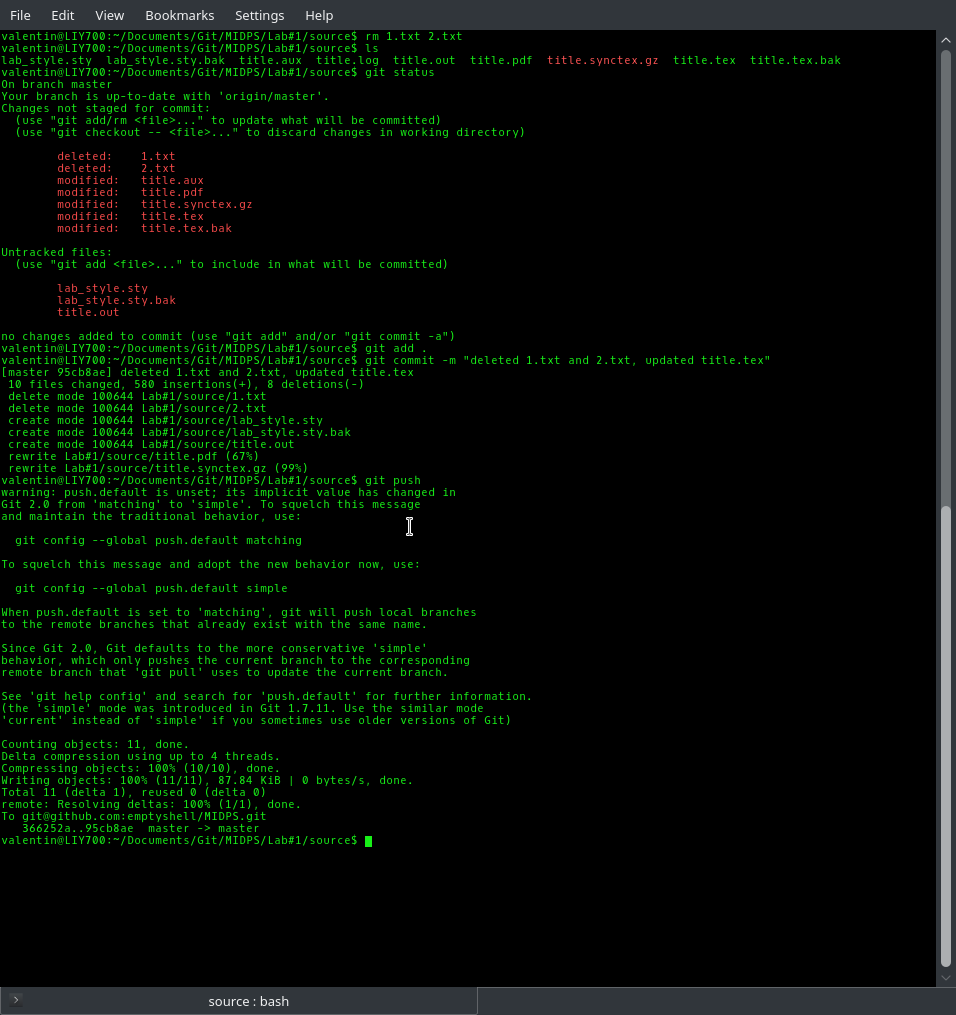
\includegraphics[height=130mm]{/home/valentin/Documents/Git/MIDPS/Lab#1/res/example}
	\end{figure}	
	\endgroup 
	\pagebreak
	\newpage
	\section*{Conclusion}
	In this laboratory work I gained skills in using github, how to create an repository and how to connect a computer via ssh key to my github account. Using command line , and especially \textbf{git} command: 
	\begin{enumerate}
		\item How to clone a repository
		\item How to add, commit and push files to repository
		\item How to create a report in latex
	\end{enumerate}
	Gained new skills in managing information in a report and create it. Created files and folders from command line and commited them to repository.
	\clearpage
	\pagebreak
	\newpage
	\begin{thebibliography}{99999}
	\singlespace
	\normalsize
	\bibitem{NaoOfficial} Aldebran Robotics, \textit{ official page}, \url{www.aldebaran.com/en}


	\bibitem{Ojala} Timo Ojala, \textit{Multiresolution gray-scale and rotation invariant texture classification with local binary patterns}, 2002

	\bibitem{biometrics} Biometric, \texttt{www.biometricupdate.com/201501/history-of-biometrics}
	\end{thebibliography} 		
\end{document}
